\begin{figure*}[h!]
\captionsetup[subfigure]{position=above,labelformat=empty,margin={1em,0em},skip=-.1em}
\centering
\begin{subfigure}[t]{.35\textwidth}
\centering
\caption{Average over tasks}
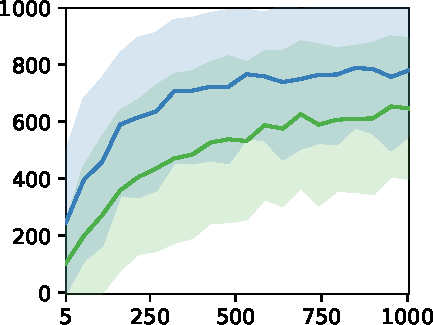
\includegraphics[width=\textwidth]{score_multi/average}
\end{subfigure}\hfill%
\caption{We compare a single \method agent trained on all tasks to individual \method agents. The plot shows test performance over the number of episodes collected for each task. The single agent learns to solve all the tasks while learning more slowly compared to the individual agents. The lines show mean and one standard deviation over 6 tasks, 5 seeds, and 10 trajectories.}
\label{fig:score_multi_avg}
\end{figure*}
